%! Author = angela
%! Date = 24/01/24
% !TeX root = ../thesis-main.tex

\chapter{Contributions}
\label{ch:contributions}
In this chapter, will be presented the main contributions of this thesis.

\section{Collektive}
\label{sec:collektive}

\emph{Collektive} is a framework designed to simplify the definition of \ac{ac} systems.

The main objective of this technology is to facilitate the development of aggregate programs that can be executed on a
variety of computing systems, such as mobile and wearable devices, computers, and the cloud.
This allows for interoperability and communication between these systems, despite their different nature.

To achieve this, \emph{Collektive} uses the \ac{fc} model to provide a straightforward and intuitive method for defining
an aggregate program, without the need for low-level coding.
In addition, \emph{Collektive} has been developed to be multiplatform, so it can be executed on different systems thanks
to the use of \emph{Kotlin Multiplatform}.

As for the feature solution of alignment for the correct functioning of aggregate programming,
it has been developed a compiler plugin with the purpose of annotating the functions that are aligned;
those paths will be used for the actual alignment of the nodes.

\paragraph{Project Structure}
The project is subdivided into different submodules (as in \Cref{fig:pacakges}), each with a specific purpose:

\begin{enumerate}
    \item \textbf{alchemist-incarnation-collektive}: contains the pieces for the Alchemist integration,
        in order to run the aggregate programs created with Collektive on the simulator.
    \item \textbf{dsl}: is the core of the project, contains the actual implementation of the logic and the \ac{ac} operators
        and relative tests.
    \item \textbf{plugin}: subdivided into:
        \begin{enumerate}
            \item \emph{gradle-plugin}: used by gradle project in order to use the \emph{compiler-plugin}.
            \item \emph{compiler-plugin}: used to keep tracks of the stack at runtime, foreach aggregate program.
        \end{enumerate}
    \item \textbf{buildSrc}: contains the main configuration for running the multiplatform project.
\end{enumerate}

\begin{figure}[h!]
    \centering
    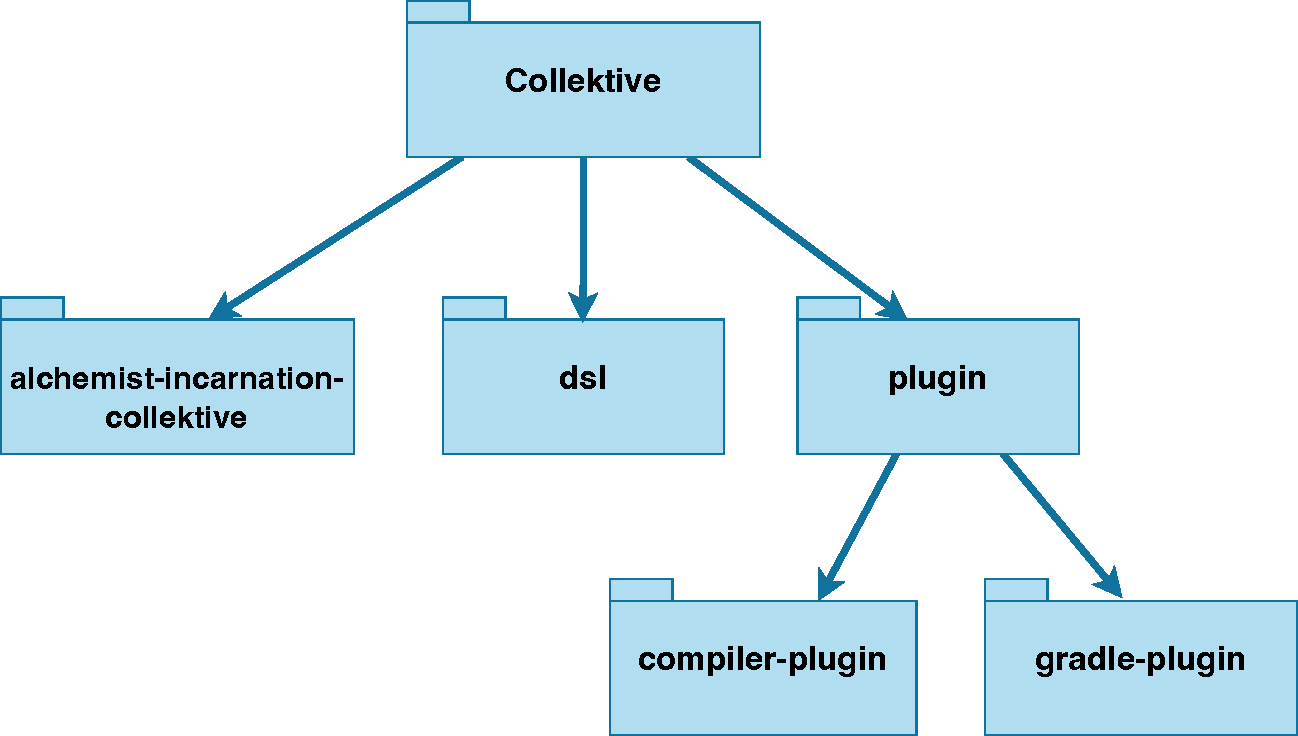
\includegraphics[width=0.7\textwidth]{figures/packages}
    \caption{Packages diagram of the Collektive project.}
    \label{fig:pacakges}
\end{figure}

Regarding the examples, there is a specific repository called \textbf{collektive-examples} that contains some samples of
aggregate programs to show how to use the \emph{Collektive} framework.

\section{DSL}
\label{sec:dsl}

In this thesis, the original implementation of the \ac{dsl} of \emph{Collektive} will be modified to allow the use of \xc{}
and to improve its performance.

%todo what is a dsl

\paragraph{Structure}
%todo add class diagrams
%For what it concerns the structure of the core of the project,
The \ac{dsl} is composed of the following components:
\begin{itemize}
    \item \textbf{Path}: represents a specific point in the \ac{ast} of an aggregate program;
    \item \textbf{State}: is an association between a path and a value, it is used by the compiler plugin to
        keep track of the computational state of the device in order to provide the correct alignment of the nodes;
    \item \textbf{Field}: represents the \emph{computational field} used by aggregate constructs.
        It is a map of messages where the key is the identifier (ID) of the node, and the value is the associated message;
    \item \textbf{Message}: is an interface that represents the message exchanged between nodes, its concept will be explained in \ref{subsec:messages};
    \item \textbf{Network}: is the interface that represents the network used to manage the communication between devices;
    \item \textbf{Aggregate}: the actual core of the \ac{dsl}.
        It is also used to handle all the data needed for the computation; for example, the \emph{localId} and the \emph{state} of the device.
        It contains the primary functions on which the language is extended, such as \texttt{exchange}, \texttt{exchanging}, \texttt{repeat} and \texttt{repeating};
        To create an aggregate program, a function must extend this interface, in this way it will be possible to use the aggregate functions.
        It is also implemented the mechanism to handle the alignment of the functions used within the compiler plugin;
    \item \textbf{AggregateOperators}: contains the implementation of the functions created using the \texttt{exchange-exchanging} functions,
        such as \texttt{share}, \texttt{sharing} and \texttt{neighboringViaExchange}.
        Moreover, it contains the mechanism to manage the alignment of the fields used within the compiler plugin;
    \item \textbf{YieldSupport}: contains the \emph{Yielding Context} and the \emph{Yielding Result} for the ``yielding''
        operations, which means that the function operates on an initial value but possibly returns a different value;
    \item \textbf{Collektive}: is the entrypoint for creating a ``Collektive'' device, it must have a specific \emph{ID} and a
        \emph{network} to manage the communication between devices.
        The effective aggregate program is identified by the \emph{compute function}, which will be executed
    \item \textbf{AggregateResult}: is the result of one evaluation of the aggregate program, it contains the \emph{localId}
        of the node, the effective \emph{result} of the computation, the \emph{messages to send} to other devices and the \emph{new state} of the device;
\end{itemize}

\subsection{XC in Collektive}
\label{subsec:exchange-in-collektive}

Thanks to the design of \xc{}, it is possible to implement the methods proposed by \emph{field calculus}
(~\ref{par:syntax-of-field-calculus}) in terms of \emph{exchange} (~\ref{par:communication-in-xc}).
The syntax of \emph{XC} allows for sending messages to specific nodes, enabling the implementation of \emph{field calculus}
operations through message exchange.

The \emph{exchange} communication is based on \emph{anisotropic} communications, meaning that it has not the same properties
or characteristics in all directions (\Cref{fig:anisotropic}); therefore, messages have custom values sent to different neighbours.

\begin{figure}[h!]
    \centering
    \includegraphics[width=0.2\textwidth]{figures/anisotropic}
    \caption{Anisotropic communication.}
    \label{fig:anisotropic}
\end{figure}

This concept can be extended to the \texttt{share} function of field calculus, with the difference that the
operation of \texttt{share} is based on \emph{isotropic} communication, meaning that properties are uniform in all directions
(\Cref{fig:isotropic}); therefore, messages have the same value sent to all neighbours.

\begin{figure}[h!]
    \centering
    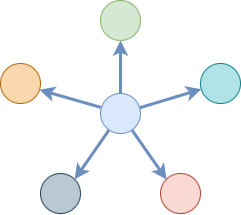
\includegraphics[width=0.2\textwidth]{figures/isotropic}
    \caption{Isotropic communication.}
    \label{fig:isotropic}
\end{figure}

All the \ac{dsl} has been modified to use \texttt{exchange} for the implementation of the other constructs such as \texttt{share}
and \texttt{nbr}, which is called \texttt{neighboring}.
Only the \texttt{rep} construct has not been implemented in terms of \texttt{exchange}, as it is a function that allows iterating
over oneself, it's better for neighbours not to receive messages of any kind, also for security and privacy reasons.
As the original implementation, it supports the evaluation of \emph{fields}.

\paragraph{Exchange}
The construct \texttt{exchange} provides
    \emph{(i)} access to neighbours' values,
    \emph{(ii)} persistence of information for subsequent executions,
    \emph{(iii)} communication with neighbours, and
    \emph{(iv)} compositional behaviour.

As seen in \ref{par:communication-in-xc}, the \texttt{exchange} function can send and return the same result, or it
can send a message and return a different result; both cases have been implemented.

%todo diagrams?

The \texttt{exchange} takes an \emph{initial} value to use as a default, and a \emph{body} that defines an aggregate
function to be computed, as seen in the code snippet \ref{lst:exchange}, returning a \emph{field}.
When executing the aggregate program, it checks which messages have been received from the neighbours and applies the function,
generating a custom value for each neighbour.

In the early stages of the design of this function, potential problems that could arise during execution were evaluated,
such as the management of initialisation, i.e.\ the first round of message exchange.
Consider a network consisting of $n$ devices, in which all are considered as neighbours to each other.
The first device ($d_1$) to start within the network will certainly have a moment when it performs its first iteration ever.

The problem arises when the device $d_1$ has not yet received any messages, so it will not have neighbour values to perform
the calculation, thus creating a deadlock situation where it does not know the neighbourhood and does not know who to actually send a message to.
For this reason, it was necessary to implement a mechanism such that the device performs a first iteration on its initial value,
and send the message to the network without a specific recipient, so that the future ``neighbourhood'' can receive it and start a communication with $d_1$.
In this way, the next devices to ``wake up'' in the network will know that $d_1$ is present and will be able to communicate with it.

\begin{lstlisting}[language=kotlin,label={lst:exchange}, caption={The signature of the \texttt{exchange} function.}]
fun <Initial> exchange(
    initial: Initial,
    body: (Field<ID, Initial>) -> Field<ID, Initial>,
): Field<ID, Initial>
\end{lstlisting}

\paragraph{Share}
The \texttt{share} construct captures the space-time nature of field computation through observation of neighbours' values,
starting from an \emph{initial} value, it reduces to a single local value given a \emph{transform} function and updating and sharing to
neighbours of a local variable, then returns the punctual value evaluated from the transformation (\ref{lst:share}).

\begin{lstlisting}[language=kotlin,label={lst:share}, caption={The signature of the \texttt{share} function.}]
fun <ID : Any, Initial> Aggregate<ID>.share(
    initial: Initial,
    transform: (Field<ID, Initial>) -> Initial,
): Initial
\end{lstlisting}

As previously introduced, this construct can be expressed in terms of \texttt{exchange}.
What \texttt{share} differs from it is that \texttt{share} does not differentiate the result of the computation based on
the neighbour that sent the message; it sends it indiscriminately to all neighbours.

\paragraph{Neighboring}

The \emph{field calculus} construct \texttt{nbr} is implemented as \texttt{neighboring}, more precisely as \texttt{neighboringViaExchange}
due to its effective implementation based on the \texttt{exchanging} function.
The \texttt{neighboringViaExchange} construct is used to access the values of the neighbours.
It takes as parameter \emph{local} (\ref{lst:neighboring}), which can be an expression or a value, and returns a \emph{field} of the same type.

\begin{lstlisting}[language=kotlin,label={lst:neighboring}, caption={The signature of the \texttt{neighboringViaExchange} function.}]
fun <ID : Any, Scalar> Aggregate<ID>.neighboringViaExchange(
    local: Scalar,
): Field<ID, Scalar>
\end{lstlisting}

%todo add something else???

\paragraph{Repeat}
The \texttt{repeat} function is the equivalent of the \texttt{rep} construct in \emph{field calculus}.
It models the state evolution over time, the value of \emph{initial} evolves at each execution depending on the \emph{transform} function,
and it returns the final value of the computation (\ref{lst:repeat}).

\begin{lstlisting}[language=kotlin,label={lst:repeat}, caption={The signature of the \texttt{repeat} function.}]
fun <Initial> repeat(
    initial: Initial,
    transform: (Initial) -> Initial,
): Initial
\end{lstlisting}

As previously mentioned, this function is not implemented in terms of \texttt{exchange}, because iterating over oneself
it is better not to send messages to neighbours, also for security and privacy reasons.

\subsection{Messages}
\label{subsec:messages}
%message modelling (in scafi there is an action that computes the messages and then creates a reaction that
%sends the message) we do it in a different way

The accurate modelling of message functionality is crucial for device communication.
Due to the different nature of messages supported, that is \emph{anisotropic} and \emph{isotropic} communication,
it has been necessary to create specific data classes for the handling of relative messages.

Previously, messages were sent to the network without considering the recipient, and the network was responsible for
delivering the message to all the neighbours that were interconnected.
Since the main feature of \texttt{exchange} is to send messages to specific neighbours with custom values, it is important
to ensure that unintended recipients do not receive the message.
Therefore, the old model of messages has been modified.

\paragraph{OutboundMessage and SingleOutboundMessage}
It has been introduced the concept of \emph{OutboundMessage} (\Cref{lst:outbound}), which is a data class that keeps track of the sender of the
message (its ID), and a map of messages, where the key is the \emph{Path} of the computation and the value is another data
class: the \emph{SingleOutboundMessage} (\Cref{lst:single}).
In this way, a device sends to the network just one \emph{OutboundMessage} that contains all the messages to send to the neighbours,
and also unburdens the payload of the network.

\begin{lstlisting}[language=kotlin,label={lst:outbound}, caption={Outbound message data class.}]
data class OutboundMessage<ID : Any>(
    val senderId: ID,
    val messages: Map<Path, SingleOutboundMessage<ID, *>>,
) : Message
\end{lstlisting}

\begin{lstlisting}[language=kotlin,label={lst:single}, caption={Single outbound message data class.}]
data class SingleOutboundMessage<ID : Any, Payload>(
    val default: Payload,
    val overrides: Map<ID, Payload>,
)
\end{lstlisting}

The main difference for the type of the communication lies in the \emph{SingleOutboundMessage} data class.
For what it concerns the \emph{anisotropic} communication, it is necessary to keep track of the identifier of the recipient
and the value associated with it, in order for the network to deliver the message to the correct neighbour.
This has been implemented with a map of \emph{overrides}, which associates to the recipient's identifier a specific value.

For the \emph{isotropic} communication, the \emph{SingleOutboundMessage} has a \emph{default} value, which is used
when there are no overrides for the recipient that is reading the messages received.

In summary, when a program is executed and a device has computed its function, it has to generate the messages to send to
the neighbours (so it's done inside the \texttt{exchange} function), it populates a \emph{SingleOutboundMessage},
that will be added to a list of \emph{OutboundMessage} and sent to the network.

\paragraph{InboundMessage}
The \emph{InboundMessage} is a data class (\Cref{lst:inbound}) modelled for the messages read from the network.
When reading the \emph{OutboundMessage}, there are some fields that are not needed, such as the receiver of the message,
which is the device itself, and is necessary to keep the default value or the override value.
To handle this, the \emph{InboundMessage} has been modelled to keep only the identifier of the sender and
a map of messages of \emph{Path} and the associated value.

\begin{lstlisting}[language=kotlin,label={lst:inbound}, caption={Inbound message data class.}]
data class InboundMessage<ID : Any>(
    val senderId: ID,
    val messages: Map<Path, *>,
) : Message
\end{lstlisting}

%\subsection{Syntax}
%\label{subsec:syntax}
%code
%rep non serve farla con xc perche non vogliamo che gli altri nodi ricevano il messaggio, cose che non gli interessano

\section{Plugin Extensions}
\label{sec:plugin-extensions}

\paragraph{Alignment}
%how

\section{Incarnation}
\label{sec:incarnation}
%how, why

%gradle task

\section{Technologies}
\label{sec:technologies}
%multiplatform

\section{Implementation}
\label{sec:implementation}
%diagrams

%dati i problemi e le scelte fatte, gli step di come è stata implementata l'exc sono i seguuenti e spiegare il codice


%todo explain the yielding thing

\begin{lstlisting}[language=kotlin,label={lst:exchanging}]
fun <Initial, Return> exchanging(
        initial: Initial,
        body: YieldingScope<Field<ID, Initial>, Field<ID, Return>>,
    ): Field<ID, Return>
\end{lstlisting}

%todo write the specific behaviour of the functions